\section{Introduction}
As previously discussed in Ch.~\ref{ch:DCR}, $\alpha$ particle backgrounds originating on or near the passivated surface of \ppc\ detectors are a major contributor to the \MJ\ \DEM\ background spectrum, but can be identified effectively via a delayed-charge recovery (DCR) pulse-shape discriminator. While \thtte\ source calibrations and \twonubb\ events can be used to estimate the DCR acceptance of bulk events, a sample of known passivated-surface $\alpha$ events are needed to estimate the $\alpha$ rejection efficiency of the analysis. Such measurements can also be used to estimate the $\alpha$ background spectral shape both before and after the DCR cut, allowing the construction of an accurate background model for the \DEM. 

Given that the weighting potential near the passivated surface varies drastically with radius (see Fig.~\ref{fig:wp_z0}), the energy lost to delayed charge in these events, and therefore the reconstructed energy of the events, is also expected to vary with radius. Similarly, the rate of charge re-release and amount of charge released, which combine to produce the DCR parameter value, are also expected to vary with radius. These variations lead to an radially- (and therefore energy-) dependent $\alpha$ rejection efficiency. The form of the DCR and energy variation depends on the mechanism of charge delay and/or loss, including whether only electrons or both holes and electrons are affected, and whether surface-charge transport or charge-trapping (followed by re-release into the bulk) near the passivated surface is primarily responsible for the observed delayed-charge effect. 

To study these effects, a collimated \am\ source was used to scan PONaMA-1, a \ppc\ detector with the same geometry as the enriched detectors currently operating in the \MJ\ \DEM. Data was taken at with the source incident at positions spanning nearly the entire diameter of the passivated surface. 

\section{Experimental Setup}
\subsection{PONaMa-1}
The detector chosen to be scanned was PONaMa-1 (serial number TP42486A), a test-run detector produced by ORTEC using natural-abundance germanium. Its production process was identical to that used for the enriched detectors in the \DEM, and its geometry is similar to that of those detectors. Its properties are given in Table~\ref{tab:PONaMA_specs}. 

\begin{table}[]
%\begin{tabular}{p{4cm} | l}
\centering
\begin{tabular}{p{5cm} | l}
\hline
\multicolumn{2}{c}{PONaMA-1 Properties} \\
\hline
Diameter & 68.9\,mm \\ 
Height & 52.0\,mm \\ 
Dimple Diameter & 3.2\,mm \\
Dimple Depth & 2.0\,mm \\
Capacitance & 1.8\,pF \\
Depletion Voltage & 1850\,V \\
Leakage Current & 10\,pA \\
Resolution at 1332\,keV \newline (Measured at ORTEC) & 1.99\,keV \\
\end{tabular}
\caption{Dimensions and operating parameters of the PONaMa-1 \ppc\ detector.}
 \label{tab:PONaMA_specs}
\end{table}

\begin{figure*}[p]
 \centering
  \begin{subfigure}[]{\textwidth}
  \centering
 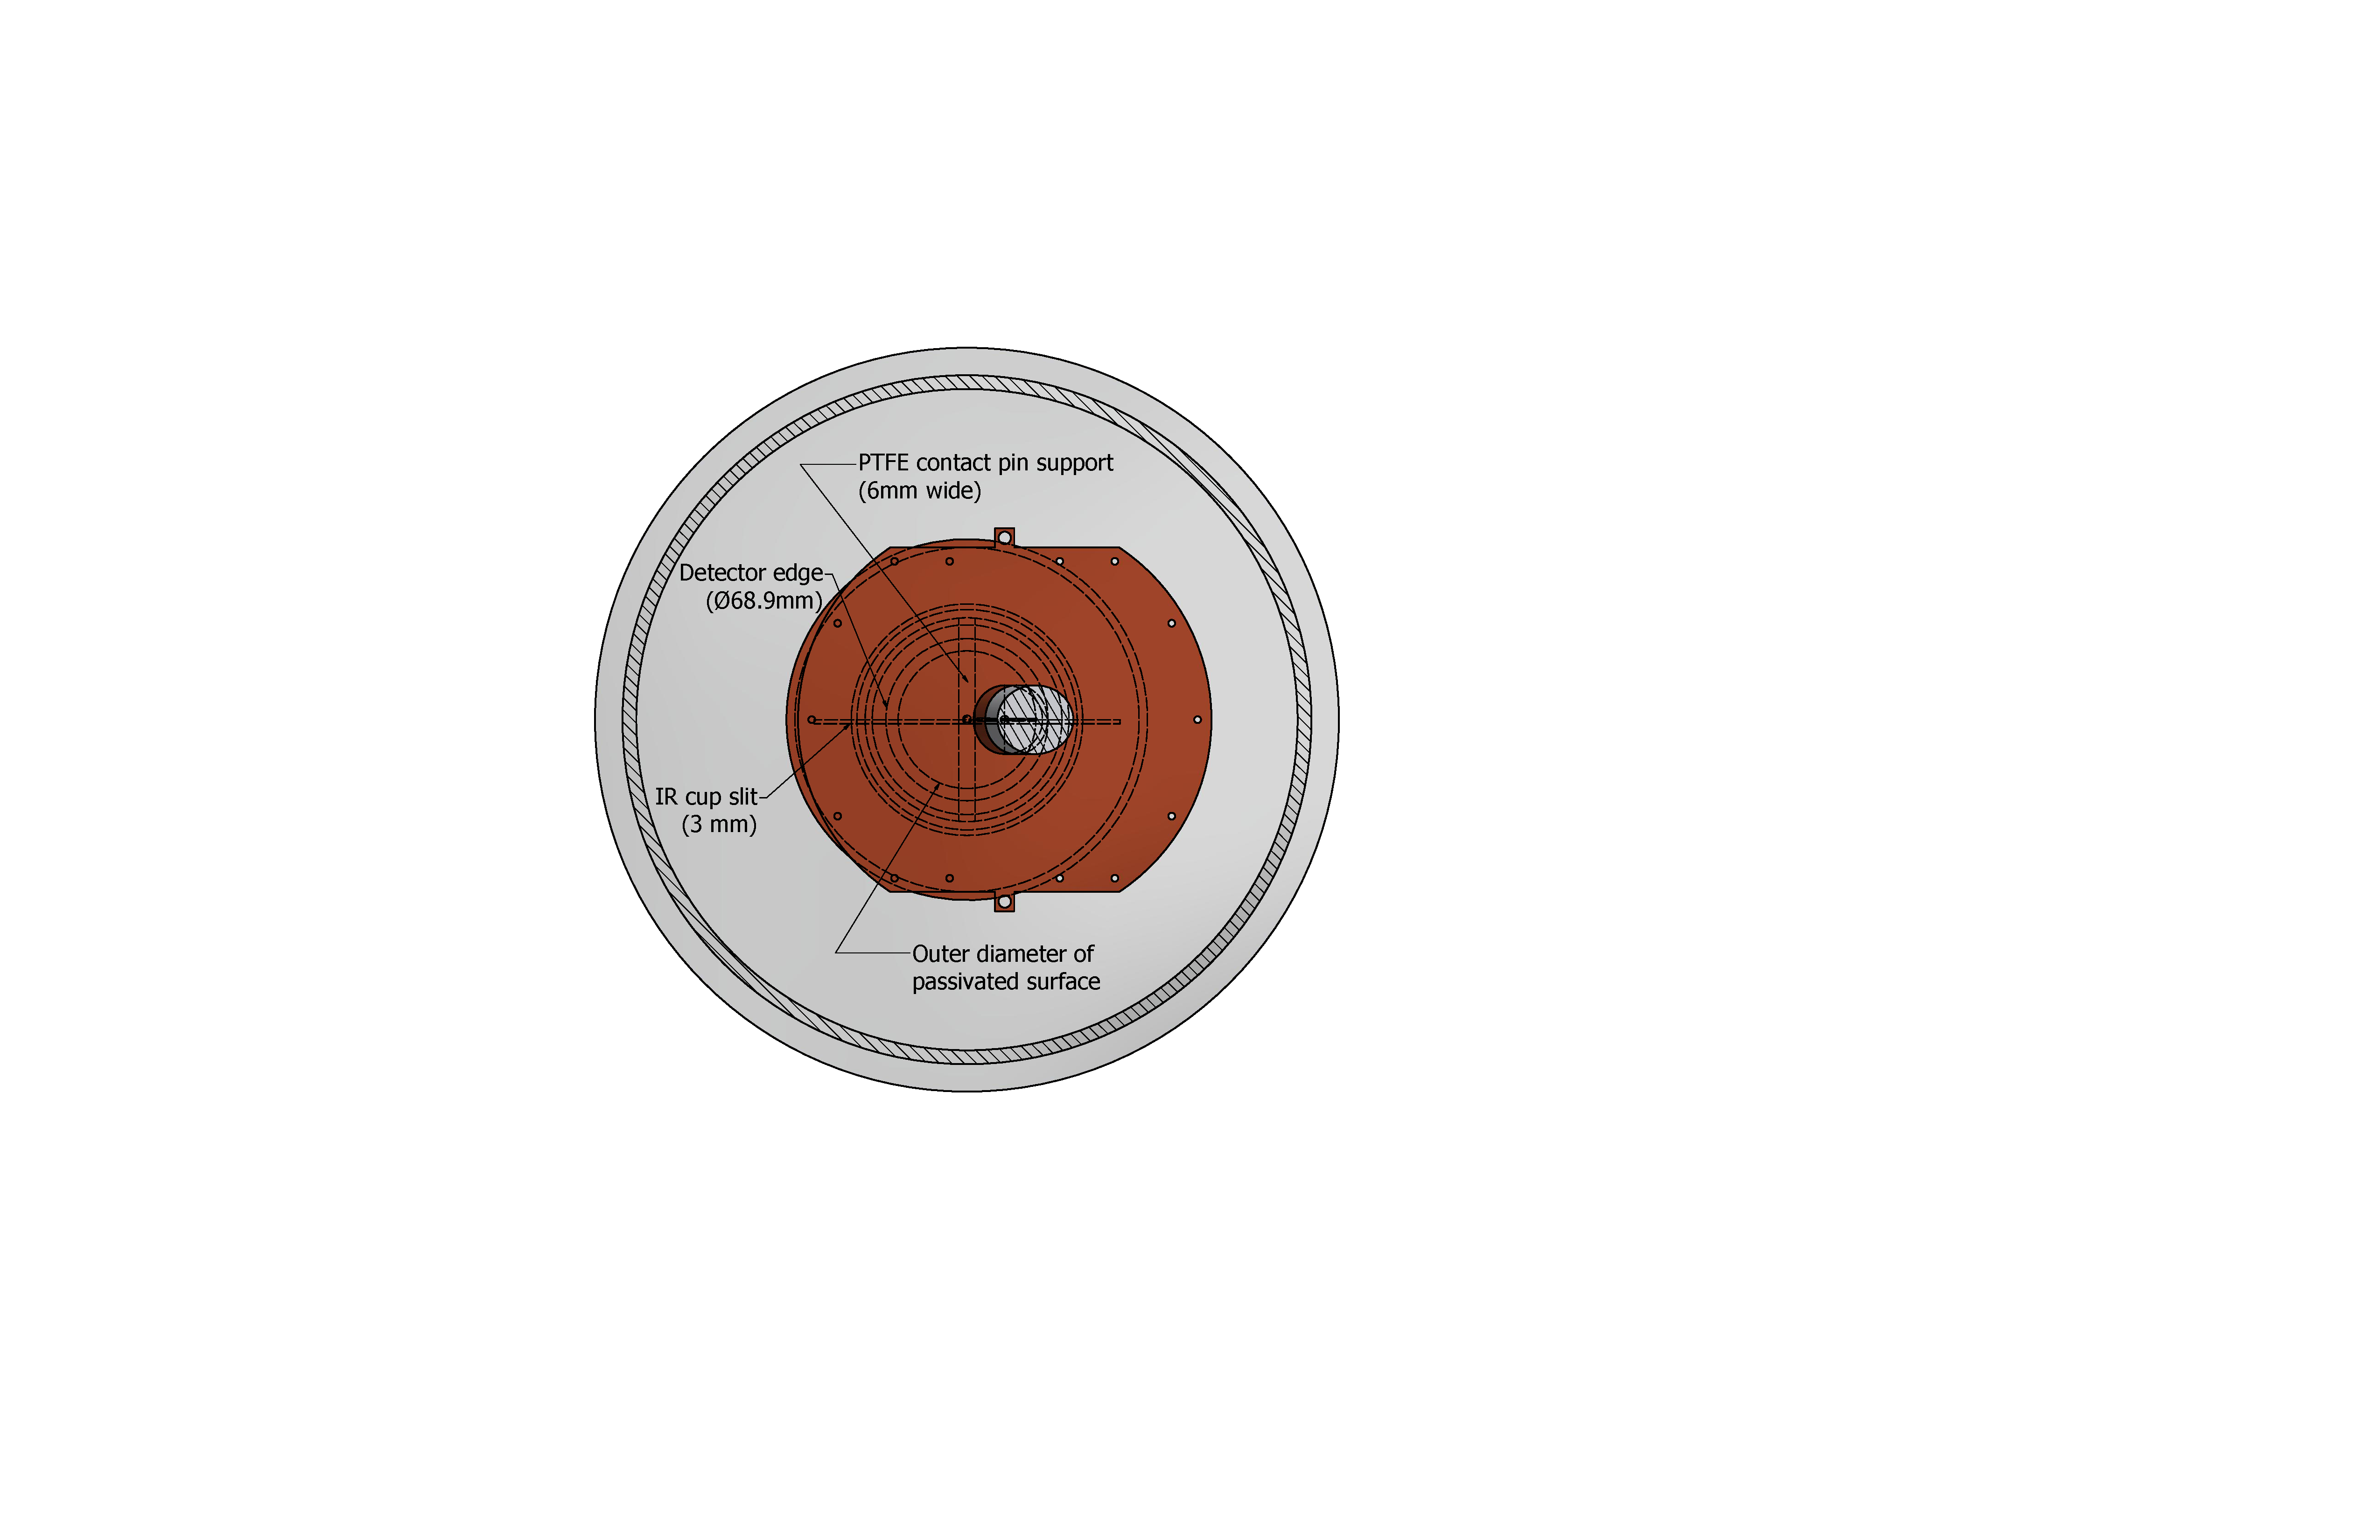
\includegraphics[height=.35\textheight]{/Users/jgruszko/Documents/Thesis/Images/Ch5/TUBE_assembly_top}
 \label{fig:TUBE_top}
\end{subfigure}
  ~
  \begin{subfigure}[]{\textwidth}
   \centering
 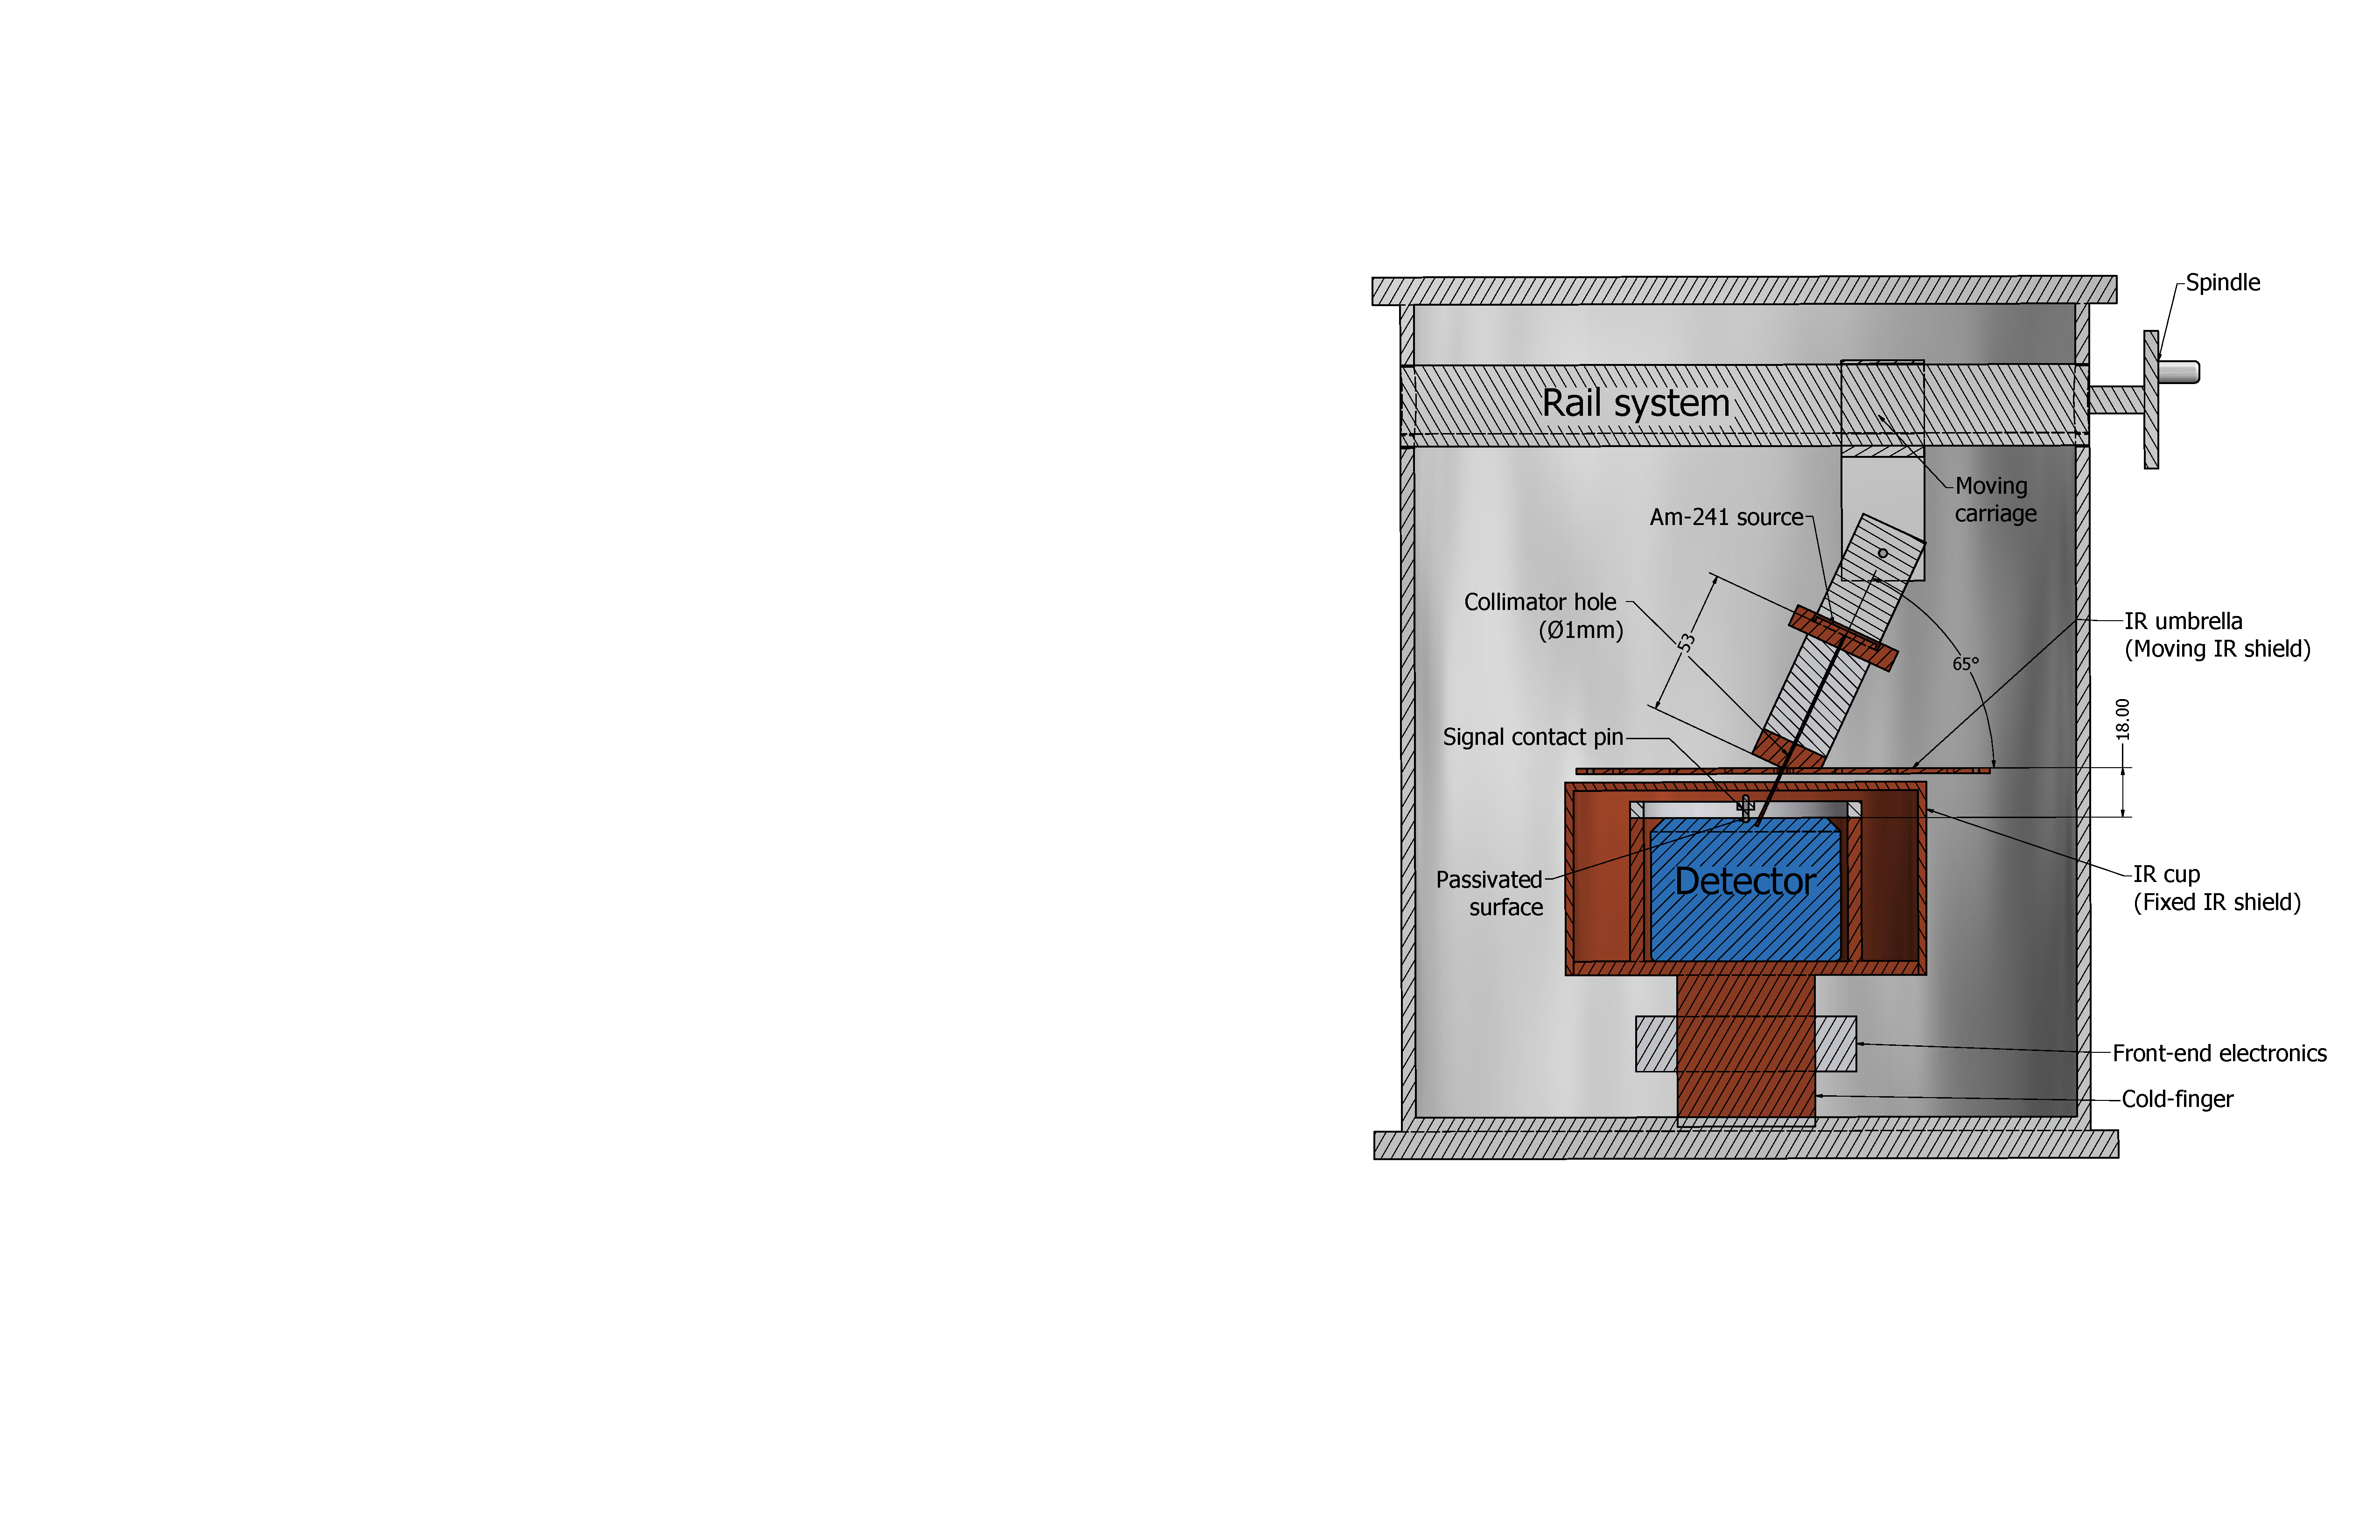
\includegraphics[height=.55\textheight]{/Users/jgruszko/Documents/Thesis/Images/Ch5/TUBE_assembly_side}
 \label{fig:TUBE_side}
 \end{subfigure}
\caption[A diagram of the TUBE scanner]{Simplified top {\it (top)} and bisected views {\it (bottom)} of the TUBE scanner, showing key dimensions. The thermal braids connecting the IR umbrella to the IR cup and the mylar covering of the IR umbrella are not shown. Details of the detector cup, front-end electronics, and cold-finger are also removed for clarity.}
\label{fig:TUBE_views}
\end{figure*}

\subsection{The TUBE Scanner}
The TUM (Technical University of Munich) Upside-down BEGe (TUBE) scanner is a custom-built cryostat first made to study the backgrounds in GERDA due to surface interactions on the p+ electrode and groove of Canberra BEGe \ppc\ detectors. It allows a \ppc\ detector to be installed ``upside-down," with the passivated surface facing upwards, so that the surface may be scanned with a collimated source. The scanner consists of three main parts, seen in Fig.~\ref{fig:TUBE_views}: the cryostat, detector holder, and collimator assembly. 

The cryostat is made from a stainless steel tube with top and bottom flanges, with a vacuum feed-through that allows the cryostat cold-finger and signal electronics (from a Canberra vendor cryostat) to be inserted. A rail system is mounted at the top of the vessel, with a rotational feedthrough on the sidewall that allows the collimator radial position to be changed while the system is under vacuum. The collimator assembly is mounted to the carriage of this rail system, which has a pitch corresponding to 1.5\,mm of travel for every turn of the spindle. Ultra-high vacuum in the vessel is achieved using a turbomolecular pumping stand with a diaphragm forepump, connected to the system by Viton-sealed flanges. The measurements described here were taken with the pump in continuous operation, though the cooled system can retain pressures of around 1E-5\,mbar even after eight hours without pumping. 

The detector is mounted in a modified version of the original TUBE copper holder, adapted for the dimensions of PONaMA-1 by the addition of teflon shims. This holder was made by adapting the vendor-cryostat detector mount, and houses the front-end electronics. Contact with the p+ electrode is made via a spring-loaded contact pin, held in a narrow Teflon\textsuperscript\textregistered holder that also provides routing for the signal cable, which runs from the contact pin to the front-end electronics. This holder creates a 6-mm ``blind spot" on the detector surface that cannot be scanned. See Figs.~\ref{fig:scan_coords} and ~\ref{fig:TUBE_photo}. 

\begin{SCfigure}
\centering
 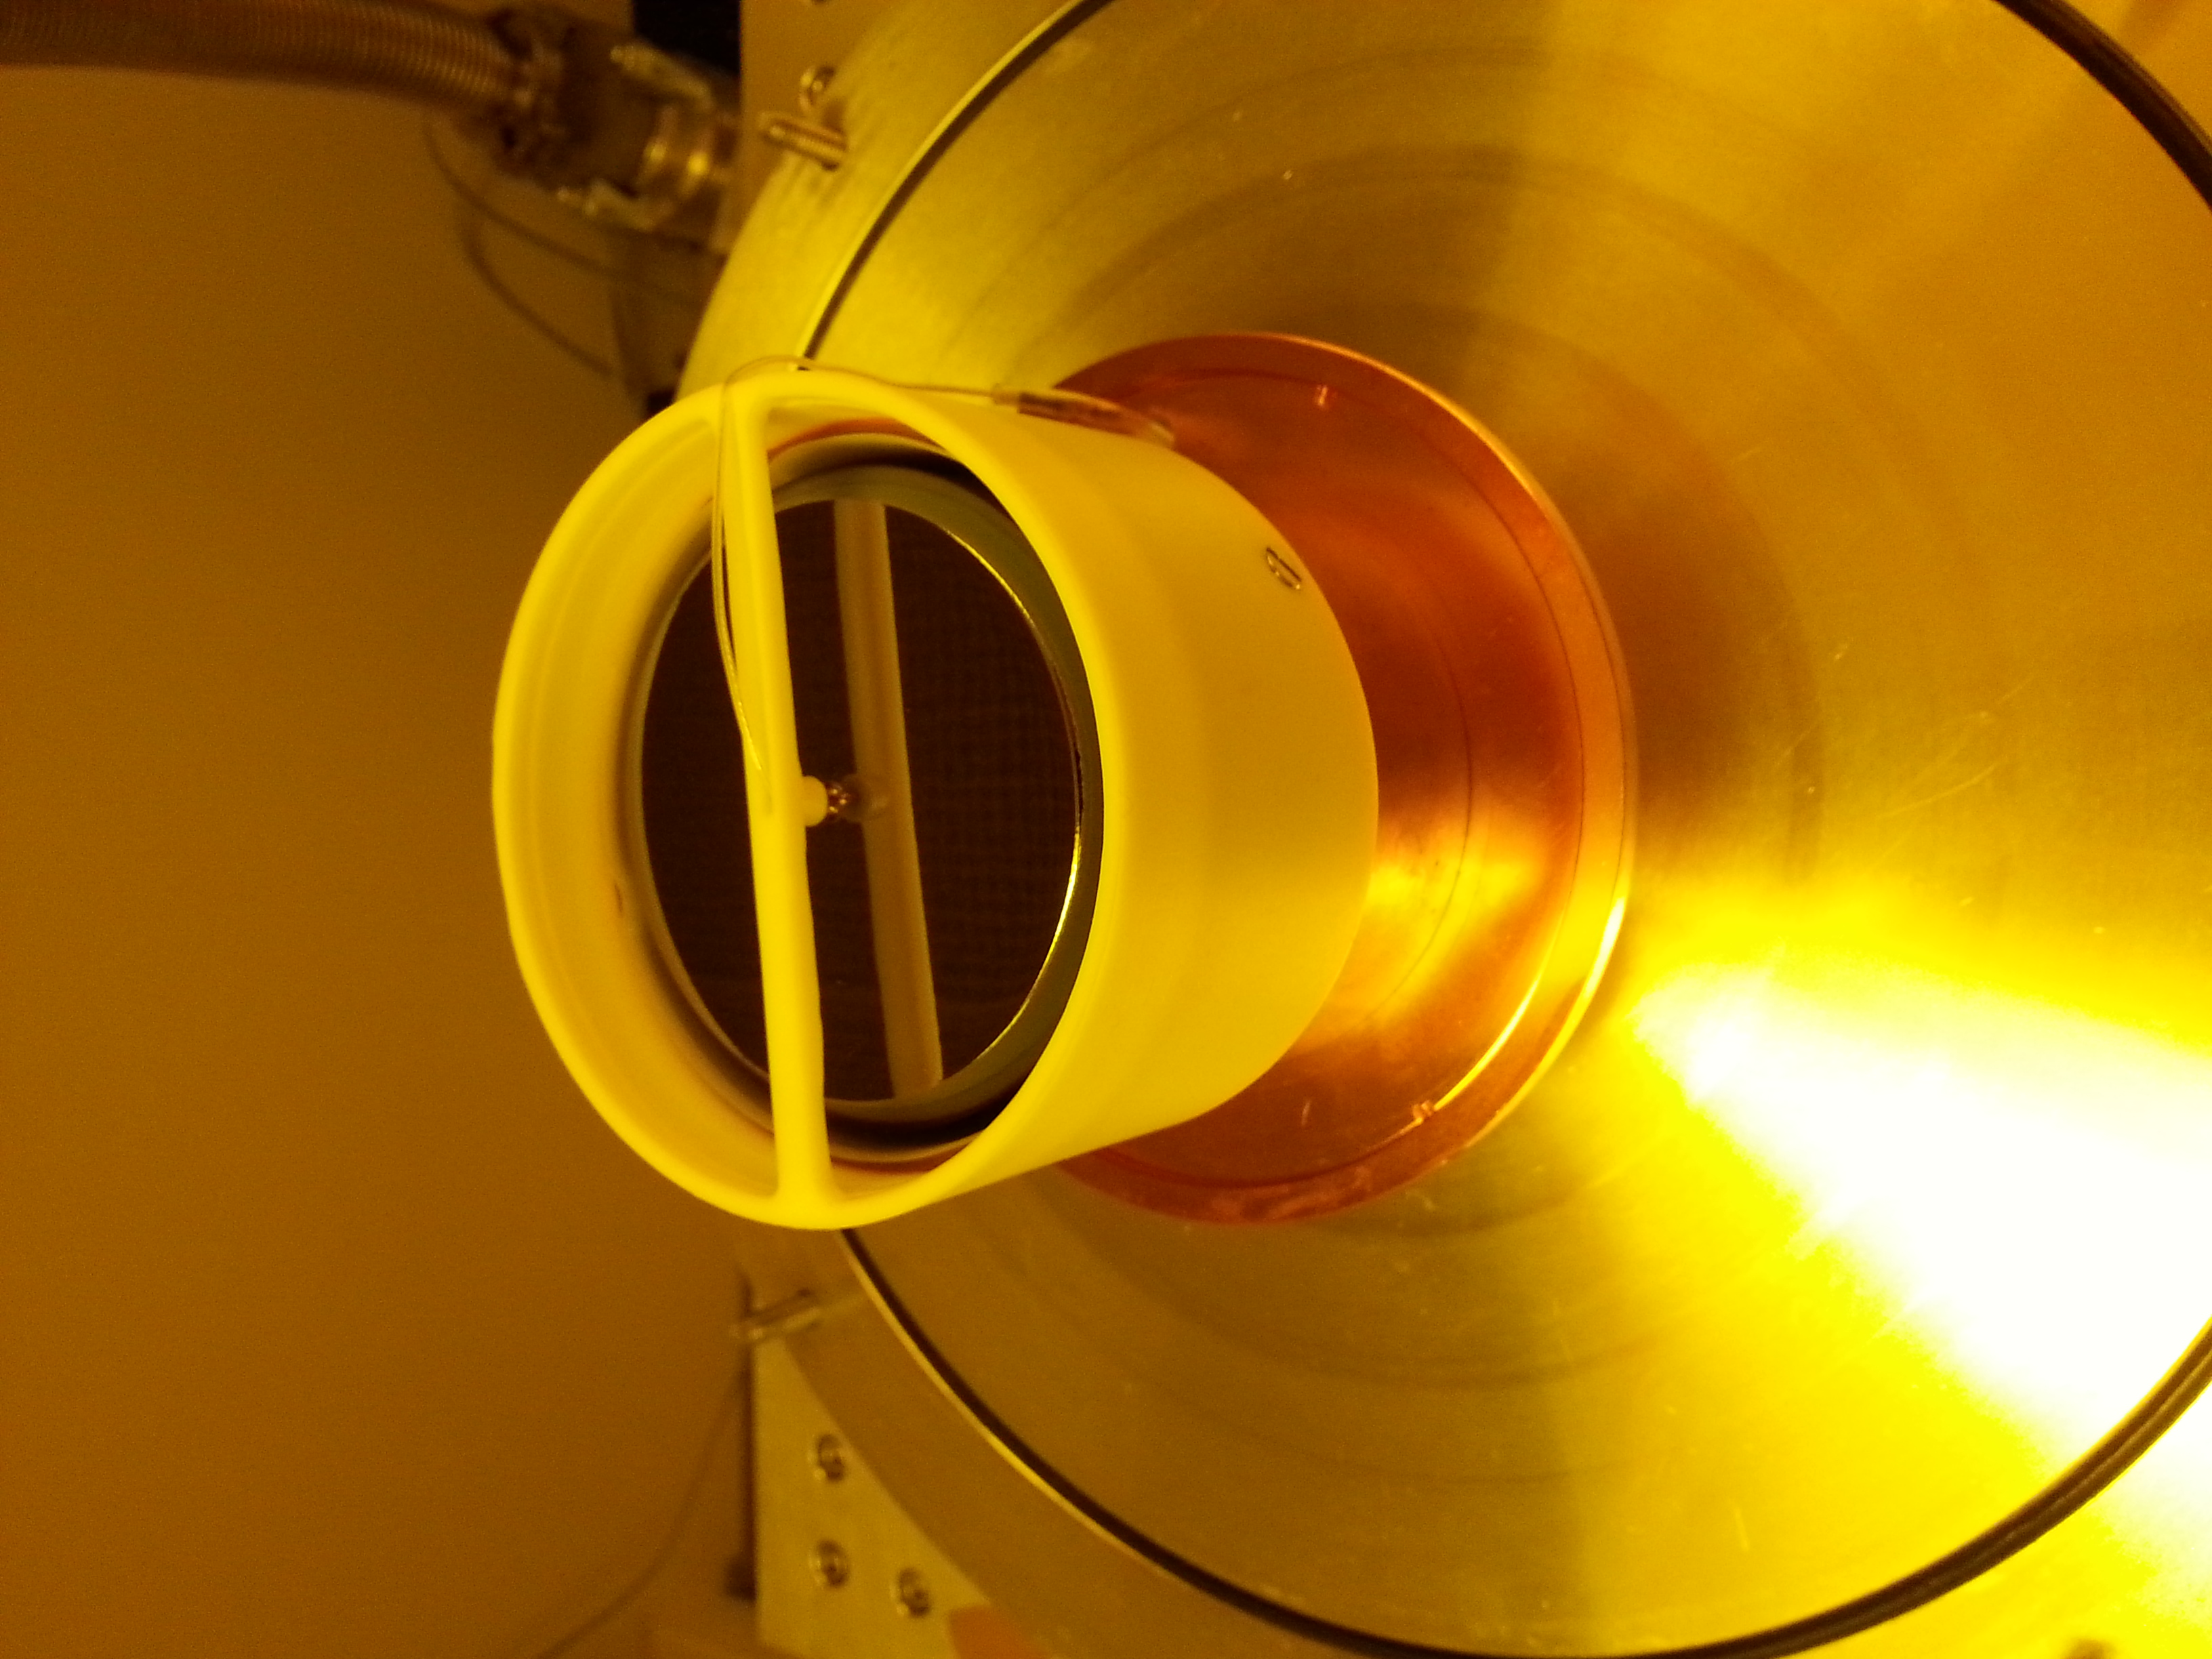
\includegraphics[height=3in, angle=270, origin=c]{/Users/jgruszko/Documents/Thesis/Images/Ch5/TUBE_detector}
 \caption[A photo of PONaMa-1 installed in the TUBE detector cup]{A photo of PONaMa-1 installed in the TUBE detector cup. The contact pin, visible at the center of the detector, is held by the Teflon\textsuperscript\textregistered\ crossbar, with the signal cable running along the top.} 
 \label{fig:TUBE_photo}
\end{SCfigure}

This assembly is housed inside a copper IR-shield (called the ``IR cup") with a 3\,mm slit running along its diameter. This slit defines the axis that is scanned along, as the source beam shines through it onto the detector surface. See Fig.~\ref{fig:TUBE_views}. 

Further IR-shielding, required due to the high IR-shine susceptibility of the large passivated surface of ORTEC \ppc\ detectors, was added for use with PONaMA-1. It is provided by a copper ``IR umbrella" shield, mounted on the tip of the collimator and moving along with the source. This shield, which minimizes the IR-shine onto the passivated surface through the slit of the IR cup, is thermally grounded to the IR cup via two flexible high-thermal-conductivity copper braids. The dimensions of the IR umbrella were subject to the existing constraint of the TUBE cryostat chamber diameter; therefore, it does not completely cover the IR cup slit at all scanning positions. This leads to variation in the detector leakage current as the collimator is moved along the surface. The top face of the IR umbrella is covered with several layers of insulator-backed Mylar\textsuperscript\textregistered, to minimize its radiative heat-load. The IR umbrella and mylar sheets have a 3\,mm diameter hole to allow the source beam to penetrate. 

\begin{figure}[]
 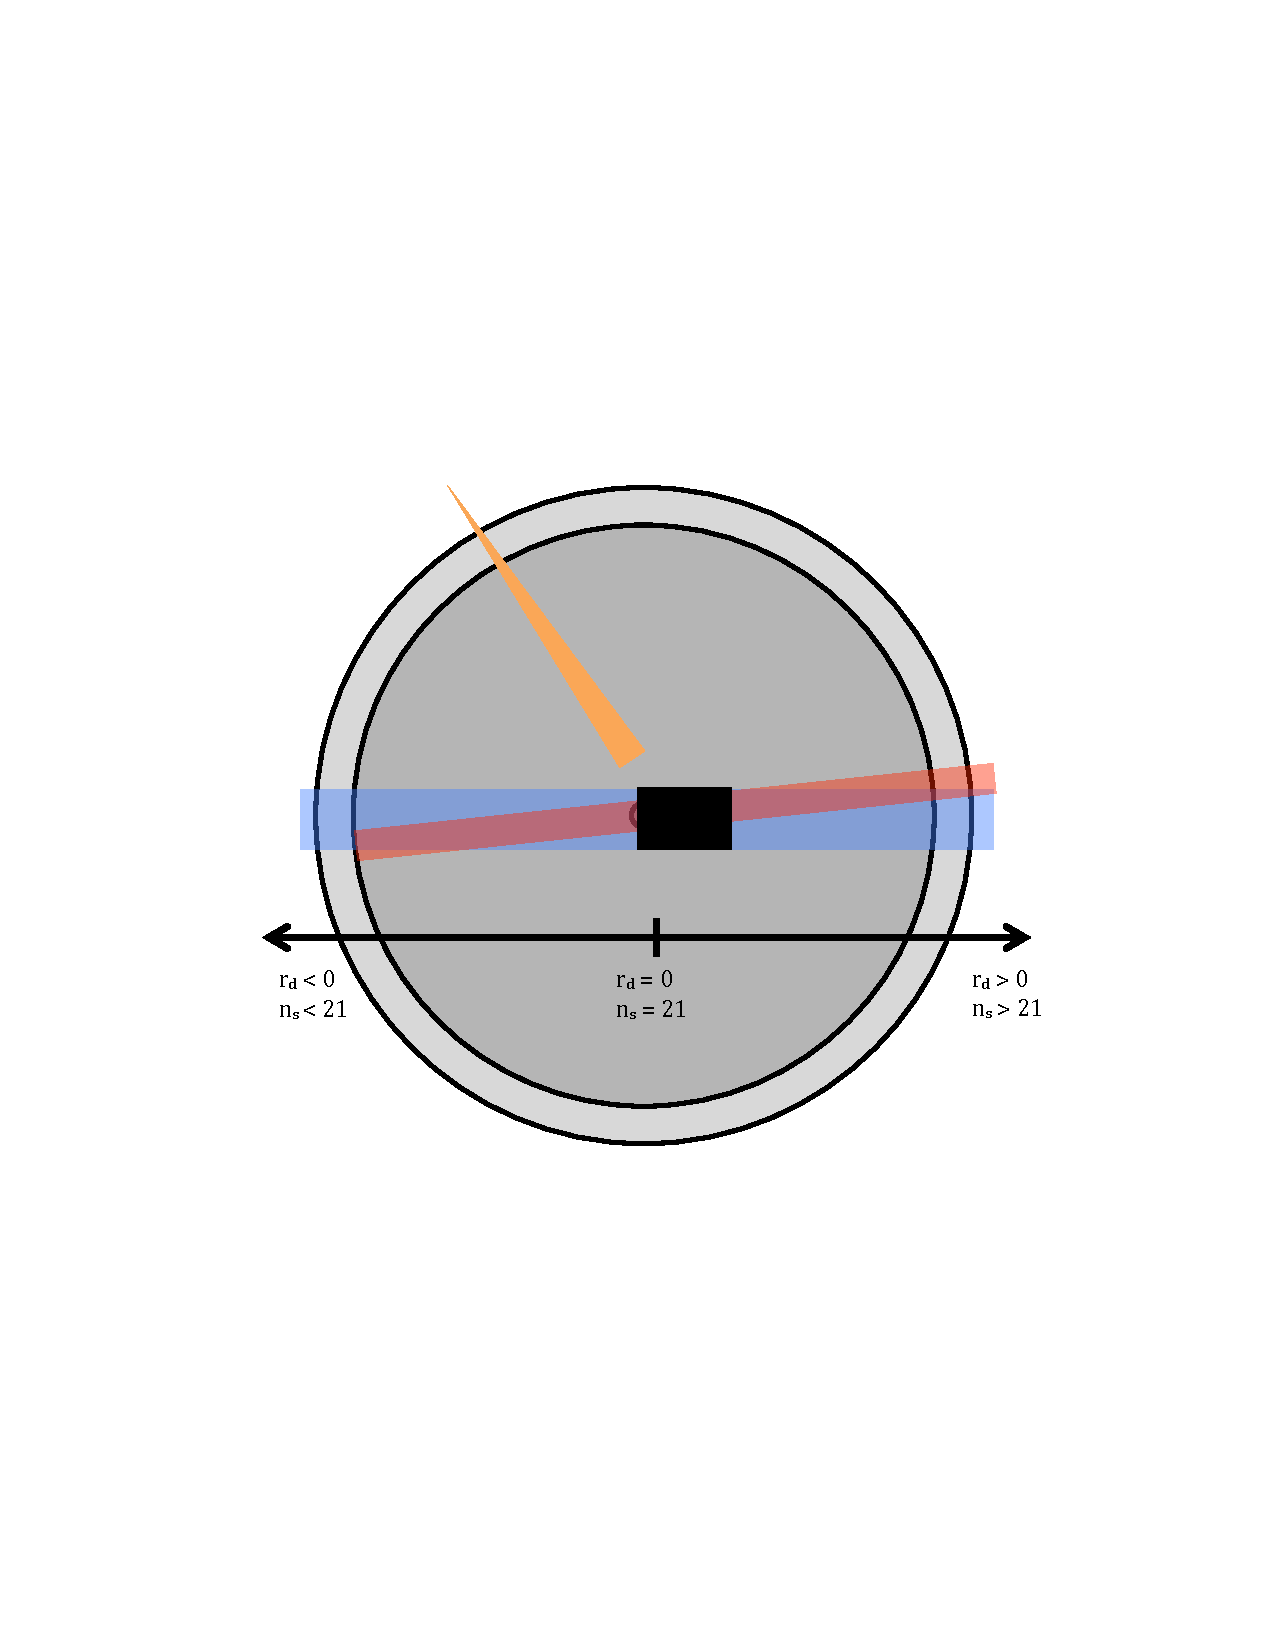
\includegraphics[width=1.0\columnwidth]{/Users/jgruszko/Documents/Thesis/Images/Ch5/coord_system}
 \caption[A diagram showing the accessible regions of the detector surface and the coordinate system of the TUBE scanner]{A diagram showing the accessible scanning regions and the coordinate systems used to describe the source position. The dark gray and light gray regions represent the passivated surface and edge of the n+ contact surface, respectively. The gold triangle represents the source beam, which forms a $66\degree$ angle to the negative r axis. The blue region represents the portion of the detector visible through the IR cup slit, and the red region is the path traced out by the source beam. Notice that due to the misalignment of the two axes, only the region of their overlap can be scanned. The black region is the inaccessible ``blind spot" due to the contact-pin holder. It occludes all but one edge of the p+ contact region, which spans the region from $r_d = -1.6$\,mm to $r_d = 1.6$\,mm. Dimensions not to scale.} 
 \label{fig:scan_coords}
\end{figure}

A photo of the TUBE scanning system (Fig.~\ref{fig:TUBE_photo}) shows the configuration of the IR umbrella, thermal grounding braids, and Mylar\textsuperscript\textregistered insulation. 

\begin{figure}[t]
\centering
 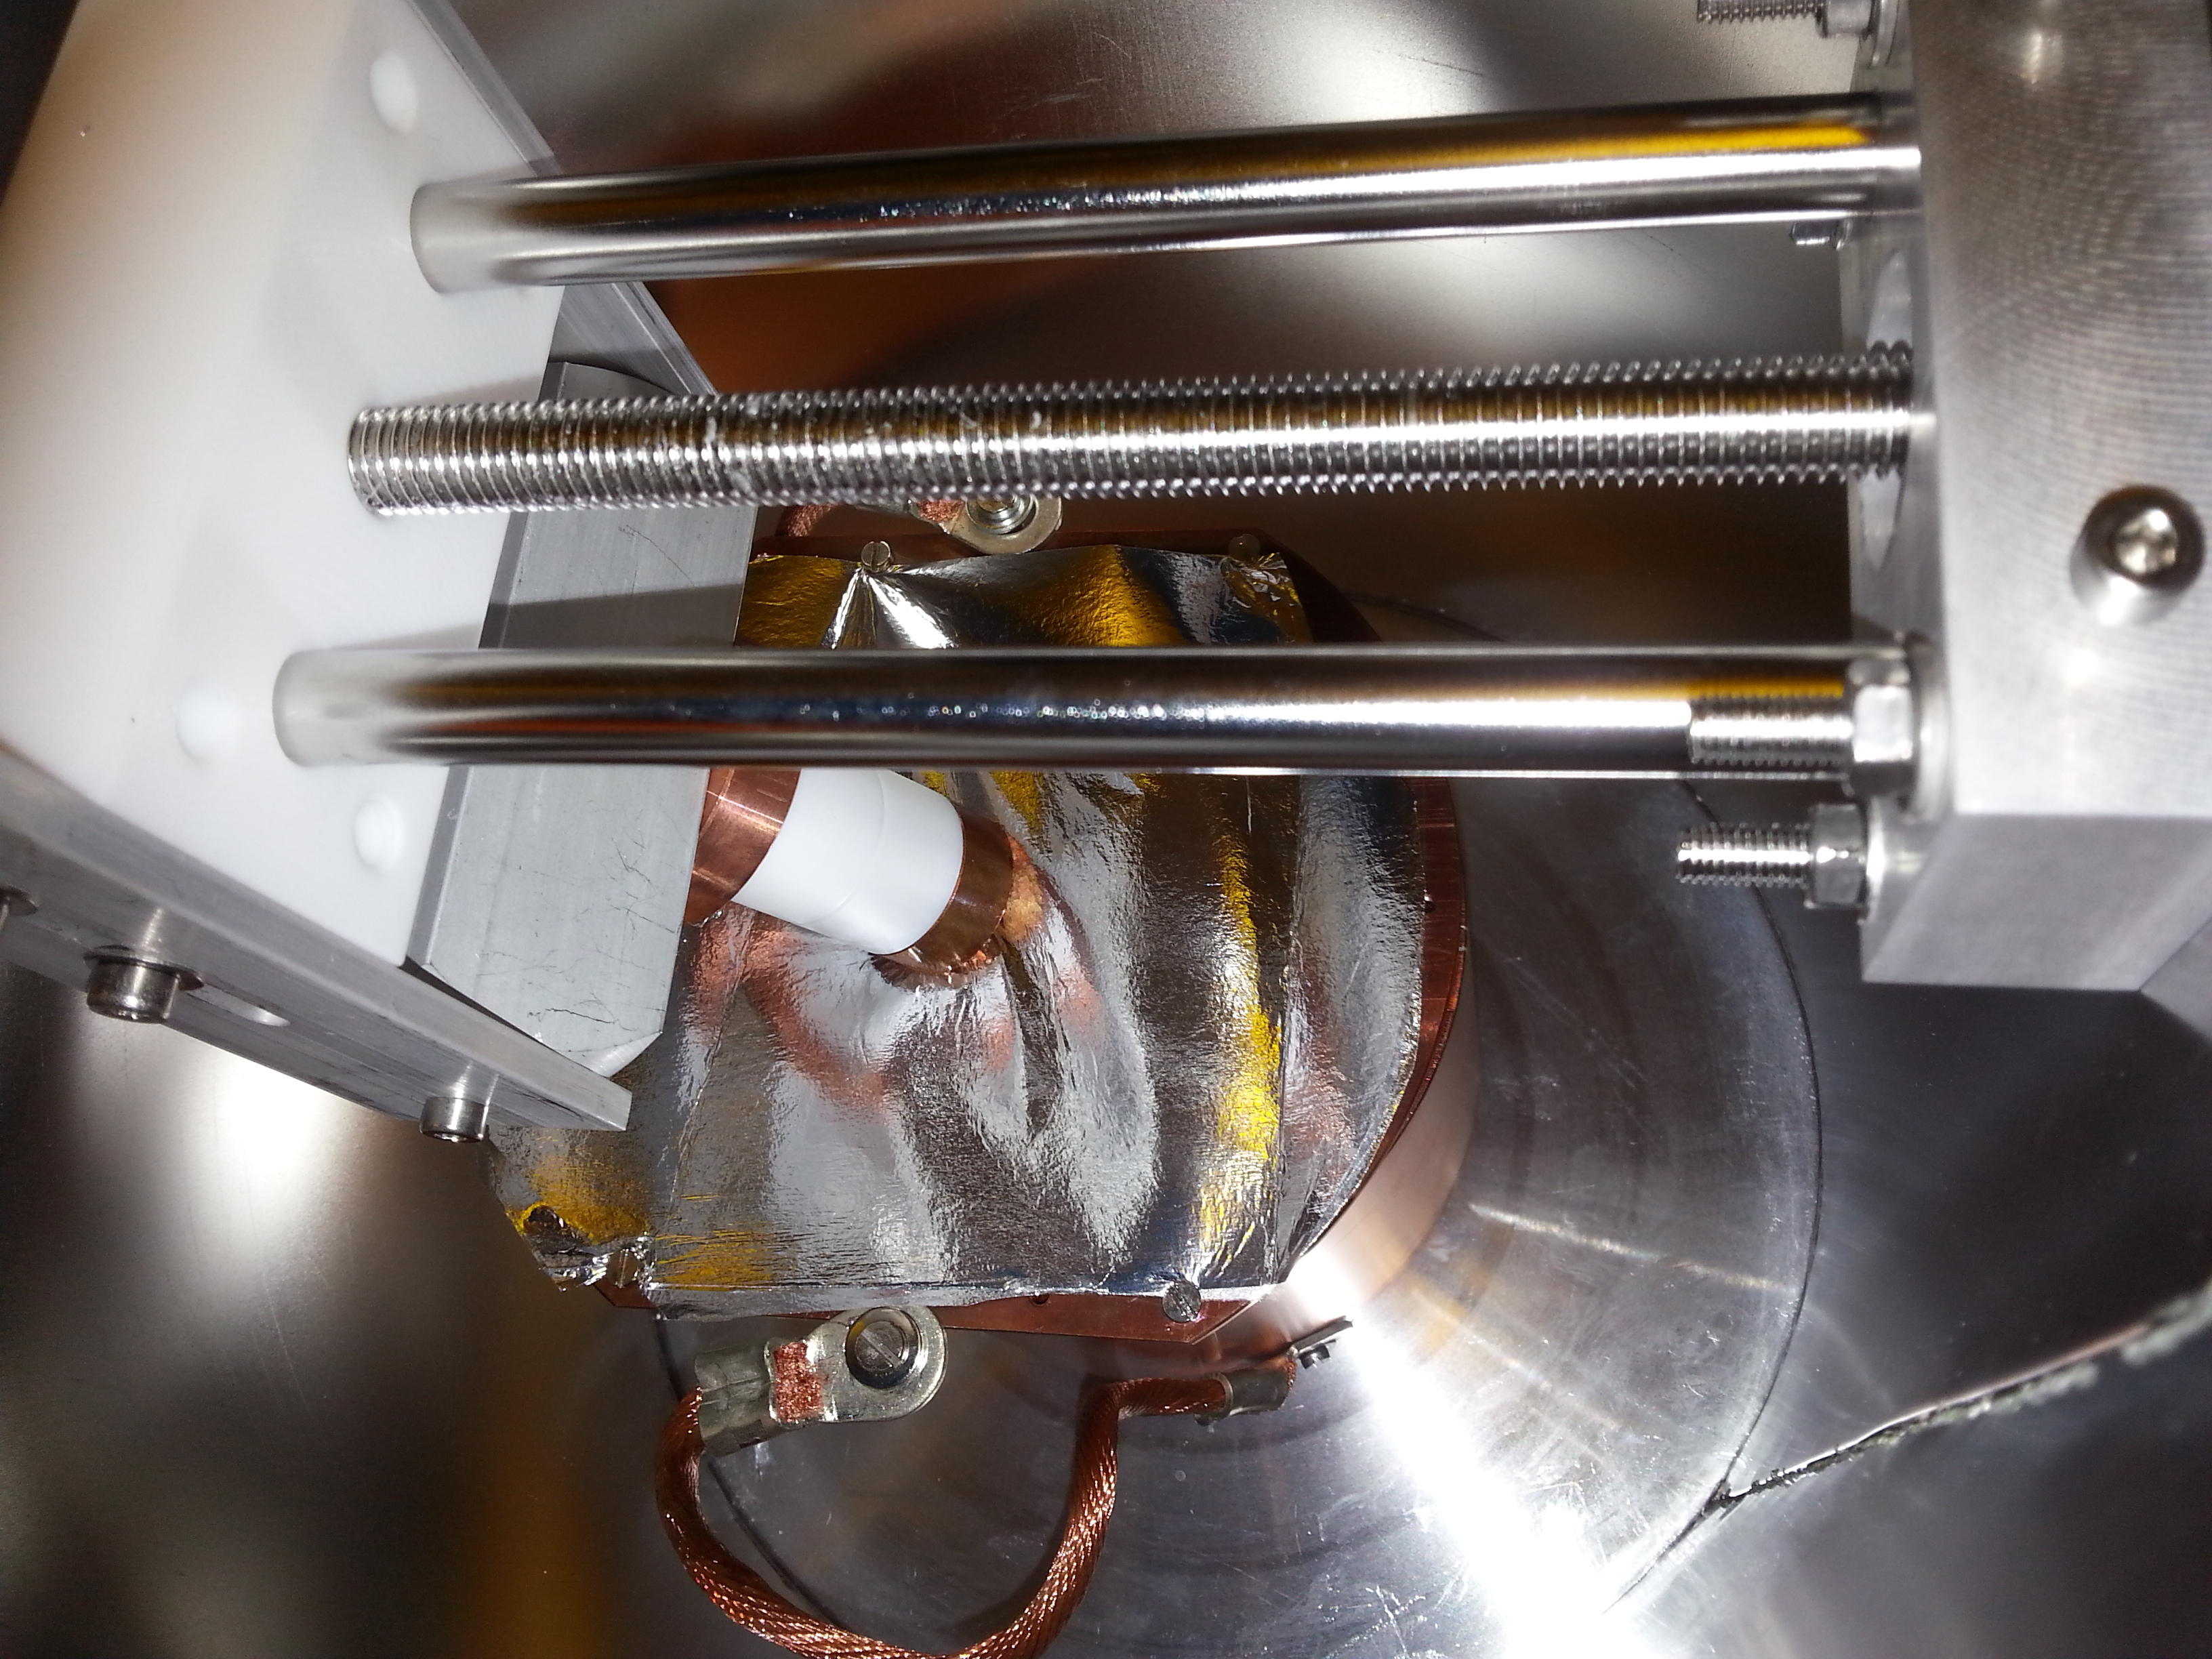
\includegraphics[height=4in]{/Users/jgruszko/Documents/Thesis/Images/Ch5/TUBE_photo_top}
 \caption[A photo of the inside of the TUBE scanner]{A photo of the inside of the TUBE scanner. The moving carriage and rail system is at the top, with the source and collimator suspended from it. The IR umbrella is suspended from the collimator tip, and is cooled via the thermal grounding braids, one of which is visible at the bottom of the photo.} 
 \label{fig:TUBE_photo}
\end{figure}

\subsection{\am\ Source and Collimator Properties}

The collimator has an overall length of 53\,mm, and is suspended from the carriage of the rail system. The source is housed in a copper holder with a 1\,mm diameter collimating hole. The beam then passes through a teflon and aluminum tube, with a collimating hole of 3\,mm in diameter, that thermally isolates the source holder, carriage, and rail system from the IR umbrella. The collimator assembly ends in a copper tip with a 1\,mm diameter collimator hole, which is chamfered to create a source-beam incidence angle of $66.8\degree$ to the horizontal plane. In the course of mounting the collimator to the rail system, this angle may change by up to $2.3\degree$ in either direction without impeding the movement of the source. For these measurements, the incidence angle is taken to be $65\degree$, as discussed in Sec.~\ref{ssec:geometry}. The spot size of the source on the detector surface is approximately 1.8\,mm in diameter. 

The \am\ source used was a 40\,kBq alpha spectrometry source provided by Eckert \& Ziegler Nuclitec GmbH, with product code AMR14. It is an open source, with the radionuclide deposited onto a 7\,mm-diameter spot of a stainless steel disc. This minimizes energy degradation, giving an expected full width at half maximum for the 5.486\,MeV $\alpha$ peak of less than 20\,keV. In the expected event rate calculation, we assume that the radionuclide is deposited with equal density over the entire 7\,mm spot.

Given the source strength and collimator geometry, an activity of 18\,mBq (i.e. 65 events/hour) is expected at the detector surface. 84.8\% of events, corresponding to an activity of 15\,mBq (54 events/hour) should include a 5.486\,MeV $\alpha$ emission. Another 13.1\% of events include a 5.443\,MeV $\alpha$ emission \cite{nudat_Am}. If the energy resolution of the detector is sufficiently reduced by interactions in the passivated surface, these peaks will be indistinguishable, and 98\% of the total activity will lie in the observed peak. 

\subsection{Muon Veto System}
The expected vertical flux of cosmic ray $\mu$ with energy over 1\,GeV is 1\,cm$^{-2}$\,min$^{-1}$ at sea level for a horizontal detector \cite{PDG2014}. Therefore the expected rate of high energy $\mu$ in the TUBE system detector is approximately 620\,mBq (2240 events/hour), far overwhelming the expected $\alpha$ event rate. An active muon veto system is used to reduce cosmic $\mu$ background rate. The veto system used consists of a 50\,cm by 50\,cm plastic scintillator panel and photomultiplier tube (PMT), placed on top of the cryostat. 

\subsection{Data Aquisition}
High voltage to PONaMA-1 was suppled by a CAEN N1471HA module. The detector was first operated at 950\,V of bias, 100\,V above the observed depletion voltage; ultimately, the bias was raised to 1050\,V to eliminate pinch-off. A Canberra Model 2002 Spectroscopy Preamplifier was used, with the low gain (100\,mV/MeV) setting in place. 

The veto system PMT was operated at a 1000\,V bias, and amplified using a Canberra Model 2025 AFT Research Amplifier, with a gain of x20 and a shaping time of .5$\mu$s. 

Data from both PONaMA-1 and the muon veto system were taken with a Struck SIS3302 digitizer, sampling at 100\,MHz. The digitizer and readout are controlled using ORCA (Object-oriented Real-time Control and Acquisition) \cite{ORCA}.

\section{Measurements Taken} \label{sec:measurements}
\subsection{As-Built Geometry} \label{ssec:geometry}
Several elements of the TUBE scanner geometry are determined at the moment of assembly, and are subject to human error. In particular, both the total vertical distance between the collimator tip and detector surface and the source beam incidence angle are approximate. Given the observed positions of the detector edges, the vertical spacing is thought to be 22\,mm (rather than the expected 18\,mm), and the angle of incidence is thought to be 65$\degree$ (rather than the expected 66.8$\degree$). 

With these as-built dimensions, the mapping from number of turns of the spindle, which is used to describe the data sets, to source spot position on the detector surface is given by $r_d = (n_s-20)(1.5\,mm)$, where $n_s$ is the number of turns and $r_d$ is the distance from the point contact on the surface of the detector. Negative and positive radii are defined as shown in Fig.~\ref{fig:scan_coords}, with 0 at the center of the p+ contact. The region between $r_d = -1$\,mm and  $r_d = 7$\,mm is occluded by the contact-pin and PTFE contact-pin holder, and cannot be scanned. The center of the point-contact is occluded by the contact pin itself. 

In the course of the measurements, it was discovered that the IR cup slit and scanning axis were misaligned. This led to a falling source rate at large-magnitude negative scanning radii, as seen in Fig.~\ref{fig:peak rate}. An additional slight sideways shift in the collimator mounting position (i.e. when aligned with the P-contact, the source shines slightly to one side of the IR-slit center line, rather than into the center of the P-contact), leads to a difference in the source obstruction at negative and positive radii. Based on the observed source rates and known geometry, the angular misalignment must be less than 2.5$\degree$, and the sideways misalignment must be less than 1\,mm. 

Hysteresis effects were observed in the source position, so an uncertainty of 0.75\,mm (corresponding to a 1/2 turn of the spindle) is assigned to all source positions. 

\subsection{Data Sets}
Data were taken at all integer-turn positions for at least 24 hours. Each of these run sets, taken without changing the source position or operating conditions, is grouped into a data set. Several multi-day runs were also taken to study the stability of the system. In those cases, multiple data sets cover the span of time, with each data set corresponding to approximately one day of run time. Scanning positions were repeated non-contiguously to study the effect of the source position hysteresis and the long-term stability of the DCR parameters. Measurements were taken at half-turn positions in the vicinity of the p+ contact and at the edges of the passivated surface.  

%\input{data_set_list.tex}

\section{Data Processing Scheme}
\subsection{Analysis Chain}
The data were analyzed using a modified version of the \MJ\ processing stream. Runs are limited to half an hour in duration and 2\,GB in file size. In practice, $\alpha$ source and background runs are half an hour long, and thorium calibration runs (whether taken with a \thtte\ or \thttt\ source) are shorter.

Each half-hour run is processed independently until the final step of processing. Using the Majorcaroot (MJOR)  and OrcaRoot software packages, the raw ORCA output files are converted into ROOT output files, which contain {\tt TTree}s of ORCA output parameters encapulated in Majorana Gerda Data Objects (MGDO) classes. Included in each run's {\tt TTree} are the raw waveforms collected by the digitizer. These waveforms are 30\,$\mu$s long and sampled at 100\,MHz, with the trigger appearing about 10\,$\mu$s after the start of the waveform. These waveforms are packaged into ``events," which contain all waveforms that triggered within a 10\,$\mu$s window. If a cosmic ray muon triggers both the veto panel PMT and germanium detector, for instance, the event will contain two waveforms. The resulting files are referred to here as ``built" data files.

The built data is then processed using the Germanium Analysis Toolkit (GAT) software package. At this processing step, each waveform has a variety of filters (such as baseline removal, pole-zero correction, etc.) and parameter calculators applied to it. Multiple waveforms in a given event are also processed in conjunction to give parameters such as multiplicity. The energy calibration (determined as described below) is applied during this stage of processing. All of the resulting values are saved to the ``reconstructed" data files, which do not contain the waveforms themselves. 

\begin{table}[]
\begin{tabular}{p{2in}| p{4in}}
\hline
\multicolumn{2}{c} {Selected Reconstructed Data Parameters} \\
\hline
Name & Description \\  \hline
{\tt run} & Run number \\
{\tt channel} & Channel (Ge or PMT) \\
{\tt timestamp} & Digitizer timestamp at time of trigger (in 10\,ns units)\\
{\tt startTime} & Start time of run (in UTC) \\
{\tt stopTime} & Stop time of run (in UTC) \\
{\tt m} & Multiplicity of event \\
{\tt pileUpWFsnRisingX} & Number of rising threshold crossings of pile-up trap. filter\\
{\tt trapEMPZ} & Maximum of baseline-removed, pole-zero corrected, trapezoidal-filtered waveform. \\ 
{\tt trapEMPZCal} & Calibrated version of the above, used for Ge energy determination. \\
{\tt onboardE} & Digitizer trap. filter energy, optimized for PMT energy determination\\
{\tt blrwfSlope} & Tail slope of baseline-removed waveform \\
{\tt mjdblrwfSlope} & Tail slope of MJD-emulating baseline-removed waveform \\
{\tt blrpzcwfSlope} & Tail slope of baseline-removed pole-zero-corrected waveform \\
{\tt TSCurrent200Max} & Current filter maximum \\
\end{tabular}
 \label{tab:GATparams}
\end{table}

A summary of the parameters saved at this stage is given in Table~\ref{tab:GATparams}. Baseline removal is applied by subtracting the average value of the first 500 waveform samples from each sample of the waveform. The pole-zero correction applied uses the decay constant $\tau = 44.224\,\mu$s, found by fitting to the decay of 1000 pulses in a calibration run from the first calibration data set taken. The trapezoidal filter used for energy reconstruction has an integration time of 8\,$\mu$s and a collection time of 3\,$\mu$s. A second trapezoidal filter, with integration time of 0.5\,$\mu$s and collection time of 0.3\,$\mu$s, is used to tag pile-up events. A one-sided trapezoidal filter, with integration time of 200\,ns and peaking time of 10\,ns, is used to calculate the current 'A' used in the determination of A vs. E (see A vs E unidoc for details). 

Three varieties of the waveform tail slope, which will be used to determine the DCR parameters, are saved. The values are the result of a two-point slope calculation, using the average value (in ADC) of the waveform in a 1\,us region for each of the points. All three varieties use the region starting 2\,us after the 97\% rise point of the waveform as the first point. The {\tt blrwfSlope} and {\tt blrpzcwfSlope} use the final 1\,us of the baseline-removed waveform as their second span. For the latter, pole-zero correction is applied before measuring the slope. The {\tt mjdblrwfSlope} parameter emulates the waveforms collected in \MJ\ data sets that do not use multi-sampling (MJD Data Sets 0, 1, and 3-5). For this parameter, the baseline-removed waveform is cut to have only 2016 samples, removing the final 10\,$\mu$s of decay tail. Then the final 1\,us of the shortened waveform is used as the second region. See Fig.~\ref{fig:tailslope}.


\begin{figure*}[]
 \centering
 %\begin{subfigure}[]{\columnwidth}
 \centering
 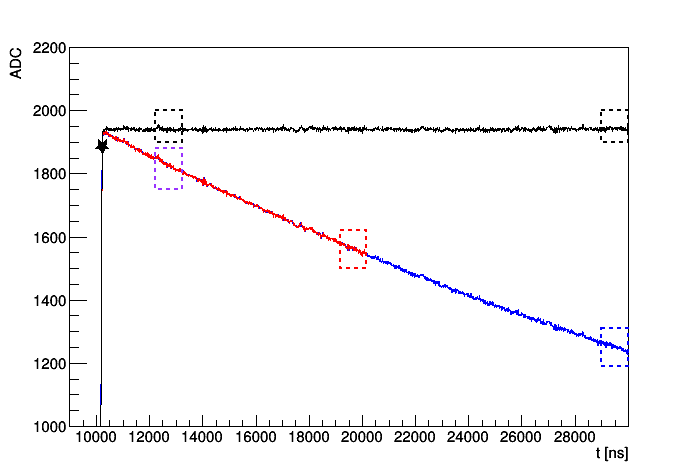
\includegraphics[height=2in]{/Users/jgruszko/Documents/Thesis/Plots/Ch5/tailslope_params_zoom_noTitle.png}
 \caption[A sample TUBE waveform, with indicated tail slope measurement points]{Sample 2614\,keV waveform, with the points needed to calculate various tail slope parameters. The star indicates the 97\% rise point of the pulse. The blue waveform has had its baseline removed; the slope between the averages in the violet and blue dotted regions is the {\tt blrwfSlope}. The red waveform has had its final 10\,us chopped following baseline removal to emulate singly-sampled MJD waveforms; the slope between the averages in the violet and red dotted regions is the {\tt mjdblrwfSlope}. The black waveform has had pole-zero correction applied after baseline removal; the slope between the averages in the black dotted regions is the {\tt blrpzcwfSlope}.} 
 \label{fig:tailslope}
% \end{subfigure}
~
% \begin{subfigure}[]{\columnwidth}
  \centering
 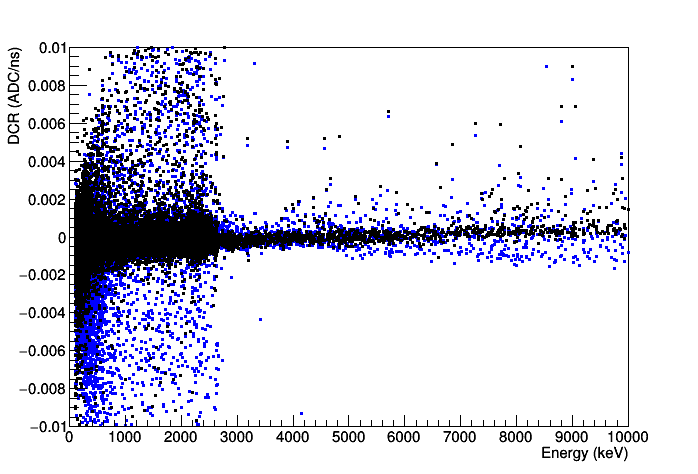
\includegraphics[height=2.5in]{/Users/jgruszko/Documents/Thesis/Plots/Ch5/dcr90_comparison_highE.png}
 \caption[A comparison of v1.0 ({\tt dcr90}) and v2.0 ({\tt dcrpzc90}) of the DCR analysis in the TUBE system]{A comparison of {\tt dcr90} and {\tt dcrpzc90} in single-site calibration events (from calibration data set 8) after the muon veto is applied. {\tt dcr90} falls and degrades in resolution at energies over 4\,MeV. Though {\tt dcrpzc90} rises slightly with increasing energy, likely due to a small change in the pole-zero decay constant $\tau$ between calibration data set 1 and 8, the effect is minimal compared to the broadening of {\tt dcr90}.} 
 \label{fig:dcr_dcrpzc_comparison}
% \end{subfigure}
\end{figure*}

In the final step of processing, GAT is used to combine about 24 hour's worth of consecutive runs into a skimmed data set. An offline energy threshold is applied to both the germanium and PMT data to reduce the number of noise events in the data set, and these thresholds are used to calculate a ``clean" multiplicity that excludes events below the analysis threshold. 

Other high-level parameters (i.e. those that require calibrated energy as an input value) are also calculated at this stage. These include A vs. E, which is the multi-site event discriminator used in this work (see A vs. E unidoc), A/E, a multi-site discriminator that is used to identify near-point-contact events, and the DCR parameters, described below. 

\subsection{DCR Parameters}
For a detailed discussion of the procedure used to calculate DCR parameters, see DCR unidoc (citation). 

Four types of DCR parameters are calculated for each PONaMA-1 waveform. For each of the parameters, versions are saved with 99\% and 90\% bulk acceptance. The {\tt dcr90} and {\tt dcr99} parameters are calculated using the waveforms after baseline-removal, with no other filters applied. The {\tt mjddcr90} and {\tt mjddcr99} parameters are derived from the MJD-emulating waveforms, which have only a 10\,$\mu$s decay tail, instead of a 20\,$\mu$s one. The are provided as a point of comparison to study the effectiveness of the DCR analysis in the \MJ\ data sets that do not use multisampling. Both of these sets of DCR parameters are calculated using the procedure described in the DCR unidoc. 

The final 2 sets of DCR parameters, {\tt dcrpzc90} and {\tt dcrpzc99}, are calculated using the baseline-removed waveform after pole-zero correction. This eliminates the need for the step in which the tail slope parameter is projected onto the energy axis, and creates a DCR parameter that has no dependence on energy for high-DCR events, unlike the other DCR parameter values. The DCRPZC parameters are a measure of the amount of delayed charge collected in the first 20\,$\mu$s after the fast, bulk charges are collected. 

The {\tt dcrpzc90} ({\tt dcrpzc99}) parameter is calculated by finding the 90\% (99\%) acceptance value of {\tt blrpzcwfSlope} for single-site non-muon events with energies between 1\,MeV and 2380\,keV, and subtracting this value from {\tt blrpzcwfSlope}. Therefore, 90\% (99\%) of bulk events should have {\tt dcrpzc90} ({\tt dcrpzc99}) $< 0$.  

The DCRPZC parameters are the most appropriate set to use when comparing TUBE results to waveform simulations, which do not include pole-zero decay. This version of the DCR analysis also performs better with respect to muon events; bulk events have consistent average DCRPZC even at high energy, while DCR degrades in resolution and falls off at energies above 4\,MeV. See Fig.~\ref{fig:dcr_dcrpzc_comparison}. Except for cases in which a direct comparison of TUBE results to \MJ\ data is required, DCRPCZ is used in this work. Ultimately, we plan to move to a similar analysis for the \MJ\ data as well, as described in the DCR unidoc. 

Additionally, normalized versions of DCRPZC, {\tt dcrpzc90norm} and {\tt dcrpzc99norm}, are calculated to correct for small instabilities in gain, PZ-decay constant, and noise in the system. To create these parameters:
\begin{itemize}
\item The {\tt blrpzcwfSlope} distribution of single-site calibration events with $1\,MeV< E < 2380\,keV$ is fit with a gaussian peak, the fit range of which is set to exclude the high-DCR tail). 
\item The centroid of the fit is subtracted from {\tt blrwfSlope}.
\item The 90\% (99\%) acceptance value is found as described above.
\item The shifted {\tt blrpzcwfSlope} values are normalized by the cut value.
\end{itemize}

Therefore, 90\% (99\%) of bulk events should have {\tt dcrpzc90norm} ({\tt dcrpzc99norm}) $< 1$, and value of these parameters is insensitive to changes in the gain of the system, unlike the unnormalized DCRPZC parameters.  

\section{Detector Performance}
\subsubsection{Energy Calibration}
Energy calibration using the GAT Multipeak Fitter (see energy Unidoc) is applied to each data set. Fourteen peaks in the spectrum ranging in energy from 295\,keV to 2614\,keV are fit with a gaussian peak, a low energy tail, a high energy tail (which fits to small values, in general), a step (which is centered at the gaussian centroid), and a linear or quadratic background (depending on the expected shape of the continuum in the peak region).

Comparing the resulting fit to a fit in which the peak positions were allowed to float, it was found that a linear calibration curve gave a poor fit to the peak positions in the spectrum. The residuals appeared to lie on a quadratic curve, with the 2614\,keV peak position being underestimated by up to 0.8\,ADC (corresponding to approximately 1\,keV). 

The fit was improved by the addition of a quadratic component to the peak position function (see Fig.~\ref{fig:calib_residuals}). I.e., the uncalibrated peak position is given by:
$$E_{ADC} = p_0 + p_1E_{keV} + p_2E_{keV}^2,$$
where $p_2$ is positive. With this change, the peak position residuals are generally less than 0.4\,ADC and are evenly distributed about 0, though some non-linearity remains, likely due to digitization effects. 

\begin{figure*}[]

 \centering
 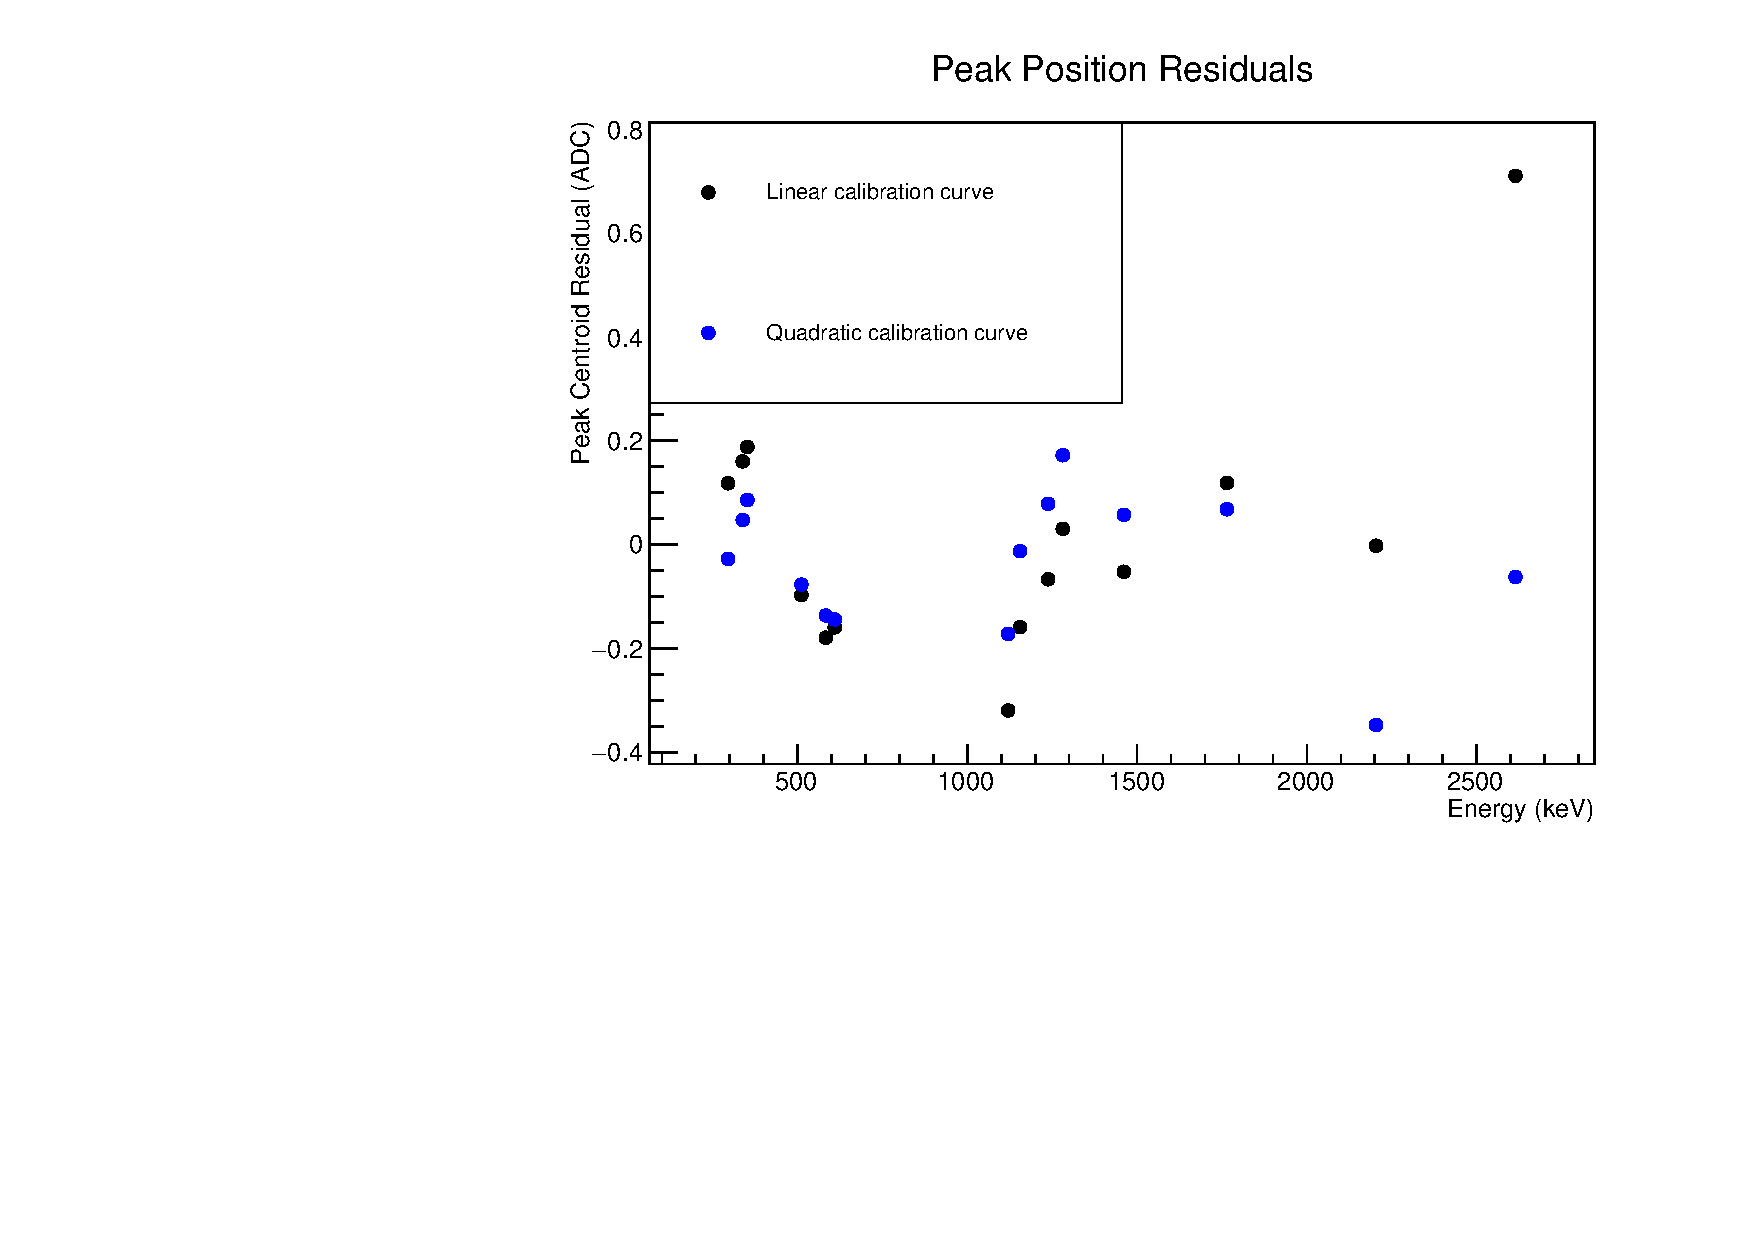
\includegraphics[height=3in]{/Users/jgruszko/Documents/Thesis/Plots/Ch5/residuals_comparison}
 \caption[The residuals of calibration peak positions]{The residuals of calibration peak positions. The entire spectrum was first fit with the peak positions (in ADC) restricted to lie either on a linear (in black) or quadratic (in blue) function of energy (in keV), and then fit with the peak positions allowed to float.} 
 \label{fig:calib_residuals}

 \centering
 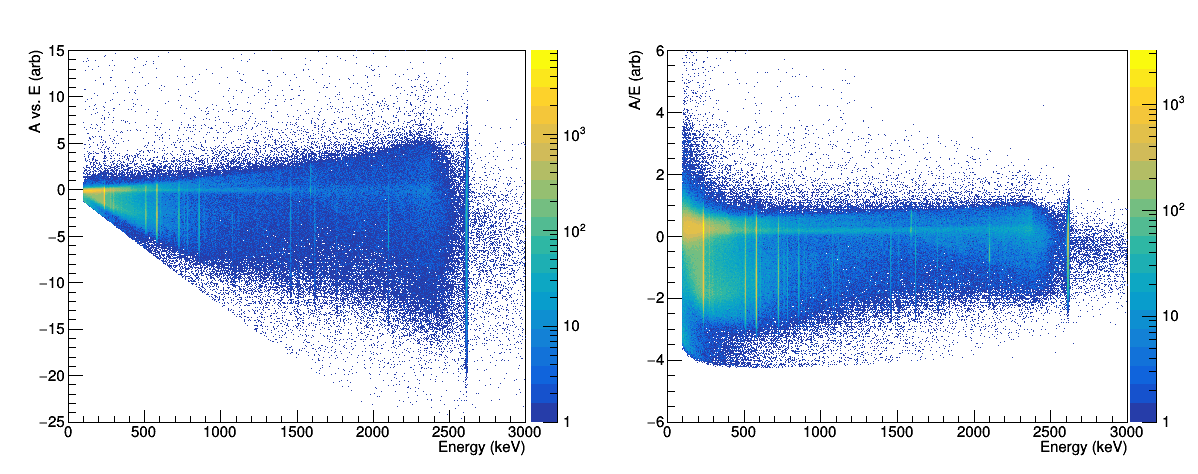
\includegraphics[width=\textwidth]{/Users/jgruszko/Documents/Thesis/Plots/Ch5/avse_aenorm_calibDS8.png}
 \caption[A comparison of A vs. E and A/E in calibration events]{A comparison of A vs. E {\it (left)} and A/E {\it (right)} in calibration events (from calibration data set 8) after the muon veto is applied. The color scale indicates the number of events. Near point-contact events have energy-dependent values of A vs. E, as seen in the sloped upper edge of the A vs. E distribution when it is drawn with respect to energy, but have energy-independent values of A/E. Therefore, A/E is used to identify near-point-contact events.} 
 \label{fig:avse_aenorm_comparison}
\end{figure*}

\subsubsection{Energy Stability}
Given the high room background rates, it is possible to calibrate every data set independently. The energy stability within data sets is measured by calculating the position of the 2614\,keV peak in ADC for each data set by applying the appropriate calibration constants, and then calculating the absolute value of the shift between consecutive data sets. The average shift is found to be $0.68\pm0.60$\,ADC, corresponding to $0.92\pm0.81$\,keV at the 2614\,keV peak. 

All shifts in the energy scale had less than a 2\,ADC effect on the position of the 2614\,keV peak save for one, between runs 1638 and 1639, which led to a shift of 4\,ADC. This shift was large enough to require that a stability correction be applied in the pulse-shape discriminating parameters. See below. 

\subsubsection{Energy Resolution}
The average FWHM at the 2614\,keV peak is $3.2\pm0.6$\,keV. The gaussian component of the peak has an average standard deviation of $1.1\pm0.1$\,keV, which would correspond to an average FWHM of $3.0\pm0.3$\,keV. The remaining contribution is due primarily to the low-energy tail, with a minimal contribution from the high-energy tail. The average resolution curve of the gaussian component is given by:
$$\sigma = \sqrt{\num{2.79e-1}+\num{3.21e-4}\,E_{keV}+\num{2.84e-9}\,E_{keV}^2}$$

The resolution suffers due to the continuous operation of the turbopump attached to the TUBE cryostat, since microphonic noise is introduced into the system. However, it was determined that the resolution was satisfactory for these measurements, and that gaining added duty cycles by avoiding pumping between measurements was a higher priority than optimizing the energy resolution. 

\subsubsection{A vs. E}
The ``A vs. E" pulse shape discriminator is used to tag and eliminate multi-site events, as described in \cite{AvsE_unidoc}. The parameters for the cut are set using $^{228}$Th calibration runs; unlike the $^{232}$Th spectrum, the $^{228}$Th spectrum has no other spectral peaks near the 2614\,keV double-escape peak (DEP), at 1592\,keV.

The current is estimated through the use of a 200\,ns {\tt TSCurrent} filter, which performs a linear fit to a small range of the waveform. The energy estimator used, {\tt trapEMPZCal}, is described above. The process used to determine the correct parameters and calculate the efficiencies and uncertainties is exactly that used for the \MJ\ analysis, which is described in the unidoc. 

To correct for the gain and noise change that occurred following run 1639, the A vs. E parameters and results are calculated separately for these two run periods. See Table~\ref{tab:AEresults}. These cuts are set using calibration data sets 1 and 8, which are 17.9 and 2.9\,hrs in duration, respectively. 



\subsubsection{A over E}
Since the width of the distribution of ``A vs. E" estimator values depends on energy (see Fig.~\ref{fig:avse_aenorm_comparison}), it is a poor choice of parameter to describe the shape of the pulses from near-point-contact alpha events. Instead, we use ``A over E," the current discriminator normalized by the energy. Using this estimator, near-point-contact events appear in an energy-independent band at higher values than single-site events. 

The A/E parameters are determined: 
\begin{itemize}
\item ``A," the maximum current, is taken to be the maximum value of a 200\,ns {\tt TSCurrent} filter.
\item The ratio A/E is calculated for all events.
\item For each of eight spectral peaks with energies from 1000 to 2220\,keV, the mean A/E value is calculated.
\item A linear function in energy is fit to the mean A/E values. This energy correction is applied to all A/E values. 
\item The A/E cut value is chosen such that 90\% of events in the DEP are accepted, following statistical background subtraction (using the sidebands of the peak).
\item The cut value is subtracted from the energy-corrected A/E value to give the ``multi-site corrected A/E" (A/E$_{corr, MS}$).
\item The 99\% acceptance value of of A/E$_{corr, MS}$ is determined. This is the value that 99\% of events (whether multisite or single-site) with energies between 1\,MeV and 2630\,keV lie below. A/E$_{corr, MS}$ is normalized by this value.
\end{itemize}

Therefore, multi-site events are expected to have A/E $<0$, and single-site events will have $A/E>0$. The final normalization corrects for gain instability and changes in the noise of the system, and 99\% of calibration-run gamma events will have $A/E<1$. Near point-contact events will have $A/E \gg 1$. 
 
As for A vs. E, the A/E acceptance in the DEP and SEP are calculated using statistical background subtraction. The region from 1989\,keV to 2089\,keV, termed the \nonubb\ region, provides an estimate of the Compton continuum reduction provided by the cut. Again, a stability correction is applied after run 1639. See Table~\ref{tab:AEresults}. 

\begin{table}[t]
%\begin{center}
\centering
\begin{tabular}{l l r r r}
\hline
PSD & Run Range &   DEP (\%) &  SEP (\%) & \nonubb\ (\%)\\  \hline
A vs. E & 1 - 1639 & 90.4  $\pm$ 2.7  & 20.0  $\pm$ 4.0  & 70.6  $\pm$ 1.1  \\
A vs. E & 1639 - & 90.1   $\pm$ 1.0  & 11.4  $\pm$ 0.8  & 50.9  $\pm$ 0.6  \\
A/E & 1 - 1639 & 90.2   $\pm$ 3.0  & 11.9  $\pm$ 1.0  & 48.7  $\pm$ 1.3  \\
A/E & 1639 - & 89.6    $\pm$ 1.9  & 12.6  $\pm$ 0.7  & 53.7  $\pm$ 0.8  \\
\end{tabular}
\caption{Multi-site discriminator survival fractions} \label{tab:AEresults}
%\end{center}
\end{table}

%\multicolumn{5}{c} {Multi-site Discriminator Results} \\
\subsubsection{Muon Veto}
The energy in the muon veto panel is estimated using the digitizer onboard trapezoidal energy filter, which is set to (rise time, integration time). An offline threshold is applied to avoid cutting on noise events in the PMT. Events in the Ge detector that occur within 10\,$\mu$s of a muon panel event are vetoed. After the cosmogenic muon cut, the event rate from 3 to 10\,MeV is reduced from 1245\,events/keV/hr to 823\,events/keV/hr. 

The relatively low muon background reduction rate is likely due to the poor noise performance of the PMT, amplifier, and energy filters. The system was not extensively tuned to optimize the energy threshold. In spite of this, the Ge spectrum of vetoed events has the expected features (see Fig.~\ref{fig:muVeto}). The reduction of the muon rate achieved is sufficient to allow measurements of the alpha source peak. 

\begin{figure}[h]
 \centering
 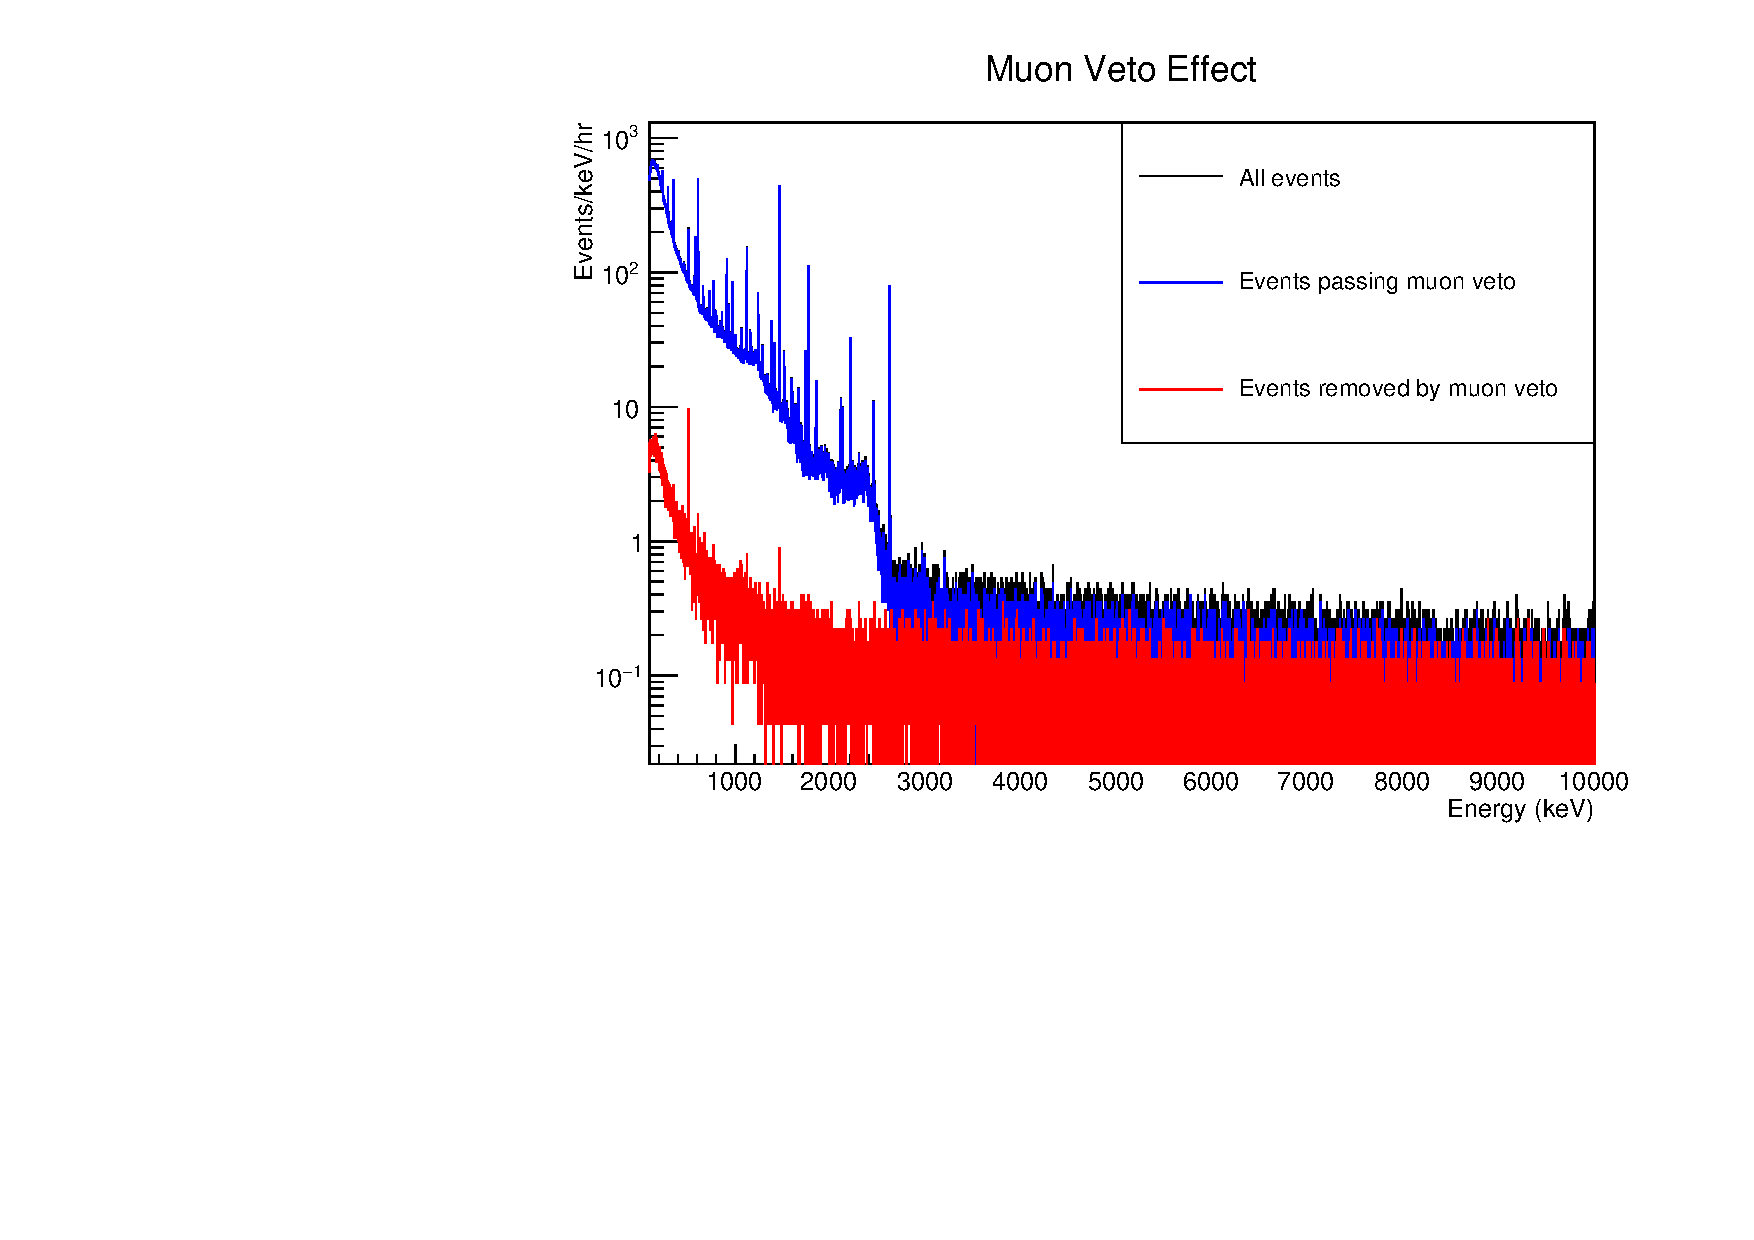
\includegraphics[height=3in]{/Users/jgruszko/Documents/Thesis/Plots/Ch5/muon_veto}
 \caption[The TUBE Ge energy spectrum, before and after the muon veto is applied]{The Ge energy spectrum, before and after the muon veto is applied (in black and blue, respectively), and the Ge spectrum of vetoed events (in red). Note that the largest peak in the veto spectrum is seen at 511\,keV, as is expected from true coincidence events due to pair production in materials near the detector, with a second small peak appearing at 1022\,keV. An additional small peak is seen at 1460\,keV, due to the high random coincidence rate of $^{40}$K events, likely from the PMT itself.}
 \label{fig:muVeto}
\end{figure}

\subsubsection{Live Time Analysis}
The dead time contributions of the Ge detector and veto system should be similar. The Ge detector triggers at approximately 60\,Hz, with a trigger window of 30\,$\mu$s and the muon veto system triggers at approximately 90\,Hz with a trigger window of 20\,$\mu$s. Each system contributes an expected dead time fraction of 0.18\%, leaving a total expected live time fraction of 99.64\,\%. 

In the the average data set used in this analysis, which is 22 hours long, the live time reduction gives 0.08\,hours (or less than 5 minutes) of dead time. 

Given the smallness of this effect compared to the statistical uncertainties in this analysis, the second-order effect of accidental coincidences is negligible, and is neglected.  

\subsection{Alpha Event Rate}\label{ssec:rate}
As a result of the as-built misalignment of the scanning and fixed IR shield axes (see Sec.~\ref{ssec:geometry}), the alpha event rate varies with scanning position. Since the degree of misalignment is not known {\it a priori}, it is estimated from the data. The fits to the energy spectra described in Sec.~\ref{ssec:E_obs} are used to find the mean energy and width of the alpha peak, and a count of the Poisson excess above the alpha-source-free runs in a 5$\sigma$ window around the peak energy is used to estimate the rate at each position. The assumption of a gaussian shaped peak in the energy spectrum is a poor one at low-magnitude scanning radii (as discussed in Sec.~\ref{ssec:E_obs}), but the rate may be estimated at larger radii on either side of these near-point contact positions, where the gaussian assumption is a good one. These results may then be extrapolated to find the rate at the remaining positions. 

As seen in Fig.~\ref{fig:alpha_rate}, the source beam is not measurably obstructed between radii of -15\,mm and 30\,mm, and falls approximately linearly at larger-magnitude negative radii. This observation, and the total reduction in rate at the largest magnitude radii lead us to derive a misalignment of less than 2$\degree$. The horizontal misalignment must be less than 1\,mm, since no scanning positions have a completely obstructed source beam. The exact values cannot be derived, since they are degenerate with one another. 

\begin{figure}[]
 \centering
 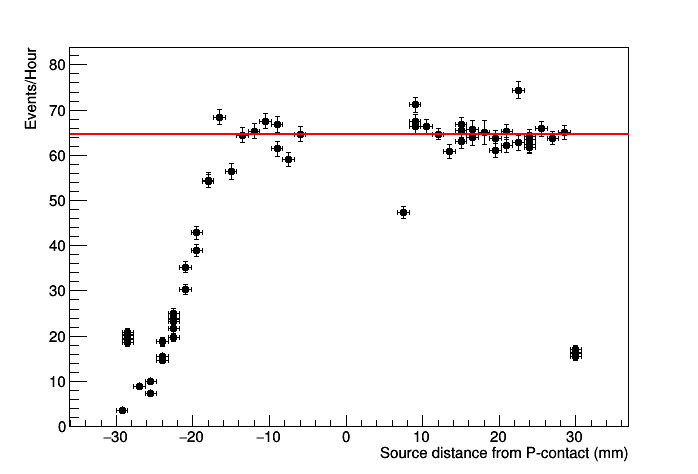
\includegraphics[width=1.0\columnwidth]{/Users/jgruszko/Documents/Thesis/Plots/Ch5/alphaRates_allPos_wAvg.png}
 \caption[Observed alpha event rates in each TUBE data set, following background subtraction]{Observed alpha event rates in each data set, following background subtraction. The red line indicates the average value, calculated as described in Sec.~\ref{ssec:rate}. The rate is reduced at positions with $r<-15$\,mm because of the misalignment of the scanning and IR cup axes. The rate at $r=7.5$\,mm is reduced by the partial obstruction of the passivated surface by the contact-pin holder, and the rate at $r=30$\,mm is low because the source beam is partially incident on the bevel, which is insensitive to alphas.} 
 \label{fig:alpha_rate}
\end{figure}

Scanning radii between -15\,mm and 30\,mm are used to calculate the observed alpha source rate. The point at $r = 7.5$\,mm is not included, since the source beam is partially obstructed by the contact-pin support at this position. The points at $r = 30$\,mm are also not included, since at this position, part of the source beam falls on the bevel, rather than on the passivated surface. The bevel is part of the n+ contact of the detector, which is insensitive to alpha interactions. Using the remaining the 32 measurements, the observed source rate is 64.6$\pm$0.5\,events/hr, or 18\,mBq.

Given that the standard deviation of the alpha event peaks (see Table~\ref{tab:E_fit_results}) is larger than the 43\,keV energy difference between the two $^{241}$Am $\alpha$ decay peaks, nearly the full activity of the source is expected to appear in the peak. Therefore, the observed activity is in excellent agreement with that expected from the source specifications and collimator geometry. 
